The methodology that provided the best results for this assignment counted the the pixels that exceeded an arbitrarily chosen threshold value of 128. 
The maximum gray scale intensity being 255, this value is the midpoint of the intensity range. 
This count was subtracted from the mean value of counts from all images in the dataset and finally squared. 
This choice of anomaly score generation proved to be reasonable. The results are presented later in the paper. 

Another method that was attempted was to uses an FFT to generate an anomaly score. This score was generated by taking the FFT of each image and then computing the power spectral density (PSD). 
After the PSD is computed, the values are scaled by the mean and standard deviation. After scaling, peaks are identified and the top four selected.
The four peaks are used to generate the anomaly score, by using their locations to compute an average location then finally the compute the distance from the origin.
This distance from the origin is the anomaly score.  

The remainder of this section will provide graphical details of the algorithm in action.
\newline
\newline
\newline
\newline
An example of two handwriting samples is shown as images in figure~\ref{fig:image1} and figure~\ref{fig:image2}. These images were produced using the imshow function from the matplotlib python library.\newline

\begin{center}
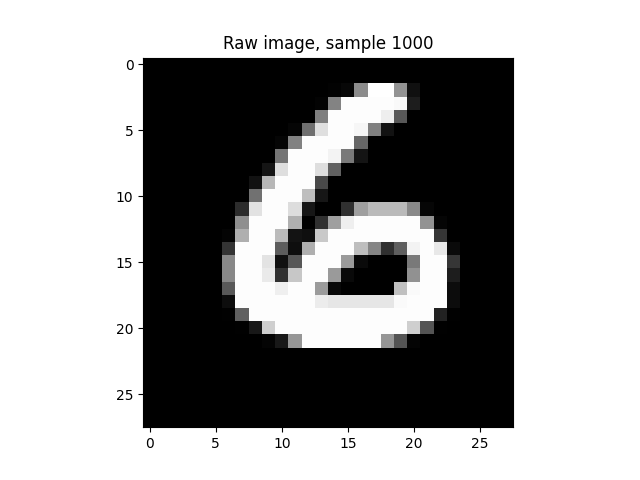
\includegraphics[width=0.35\textwidth]{image1.png}
\captionof{figure}{Handwriting Sample 1000\label{fig:image1}}
\end{center}

\begin{center}
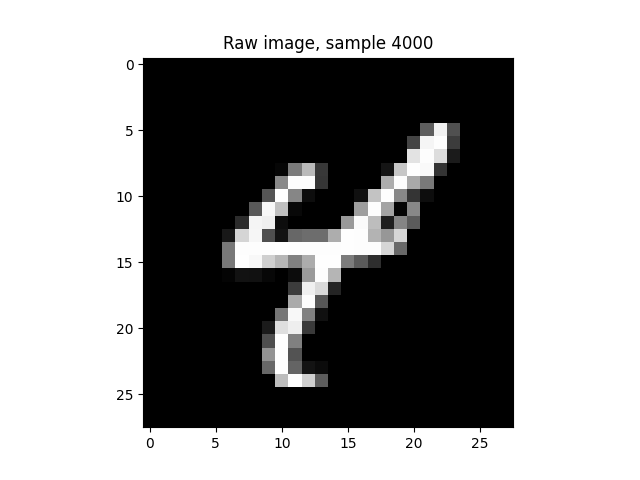
\includegraphics[width=0.35\textwidth]{image2.png}
\captionof{figure}{Handwriting Sample 4000\label{fig:image2}}
\end{center}

The first step is producing a thresholded image of each sample as shown in figure~\ref{fig:image3} and figure \ref{fig:image4} . Experiment 1000 resulted in 615 black pixels and 169 white pixels. Experiment 4000 resulted in 705 black pixels and 79 white pixels.

\begin{center}
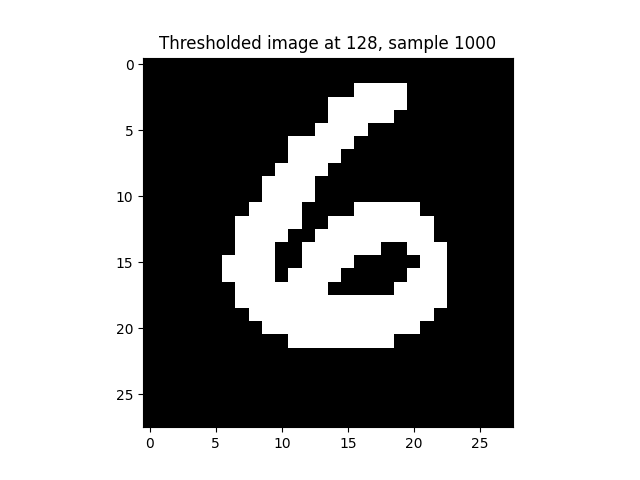
\includegraphics[width=0.35\textwidth]{image3.png}
\captionof{figure}{Threshold set to 128 of handwriting sample 1000\label{fig:image3}}
\end{center}

\begin{center}
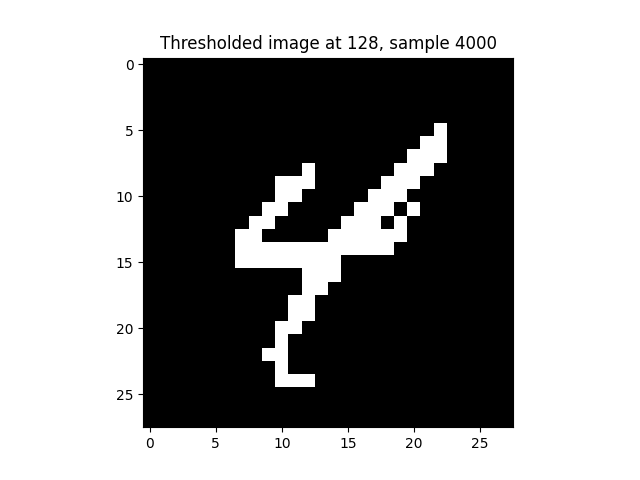
\includegraphics[width=0.35\textwidth]{image4.png}
\captionof{figure}{Threshold set to 128 of handwriting sample 4000\label{fig:image4}}
\end{center}

Then a mean image is produced, figure~\ref{fig:image5}, to generate the mean count.
The count of white pixels for the thresholded mean image is 38, figure~\ref{fig:image6}.

\begin{center}
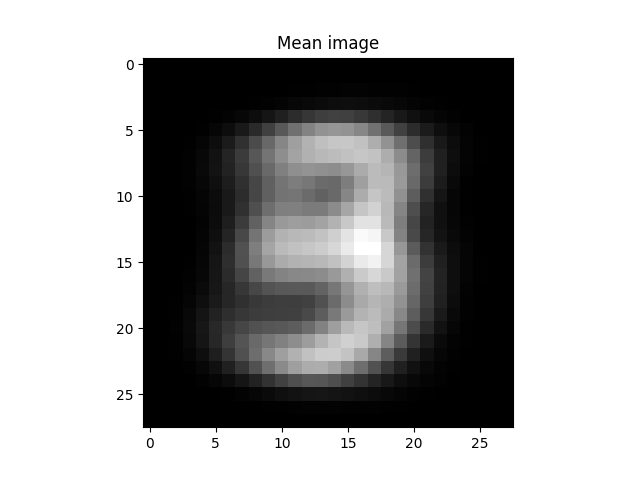
\includegraphics[width=0.35\textwidth]{image5.png}
\captionof{figure}{Mean Image\label{fig:image5}}
\end{center}


\begin{center}
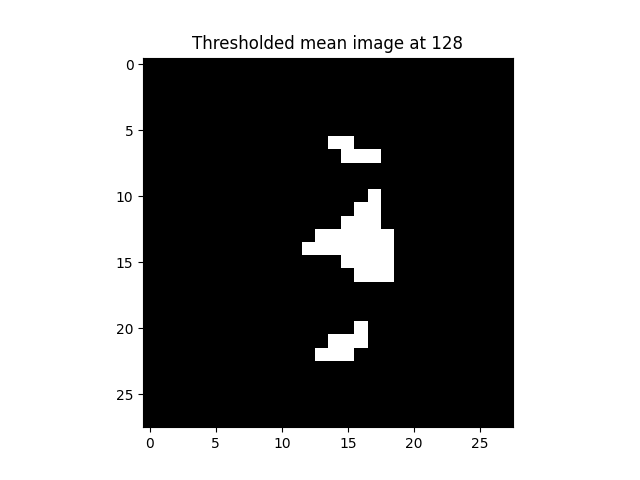
\includegraphics[width=0.35\textwidth]{image6.png}
\captionof{figure}{Threshold set to 128 of mean image\label{fig:image6}}
\end{center}

The next step requires subtracting the experiment data from the mean data. The graphical results are shown in figure~\ref{fig:image7} and figure~\ref{fig:image8}.

\begin{center}
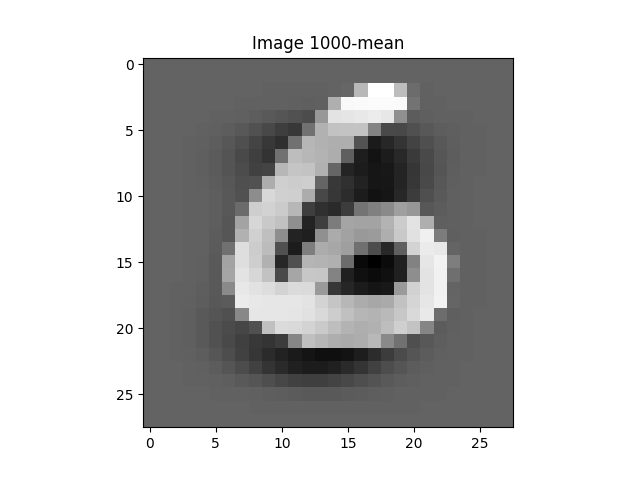
\includegraphics[width=0.35\textwidth]{image7.png}
\captionof{figure}{Subtraction of experiment image and mean image for experiment 1000\label{fig:image7}}
\end{center}

\begin{center}
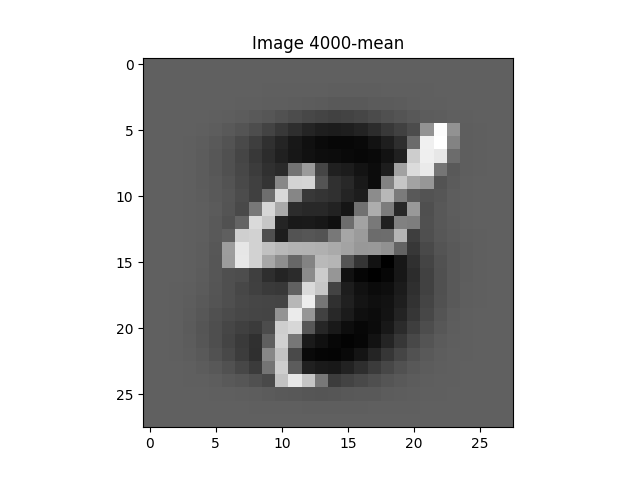
\includegraphics[width=0.35\textwidth]{image8.png}
\captionof{figure}{Subtraction of experiment image and mean image for experiment 4000\label{fig:image8}}
\end{center}

\begin{center}
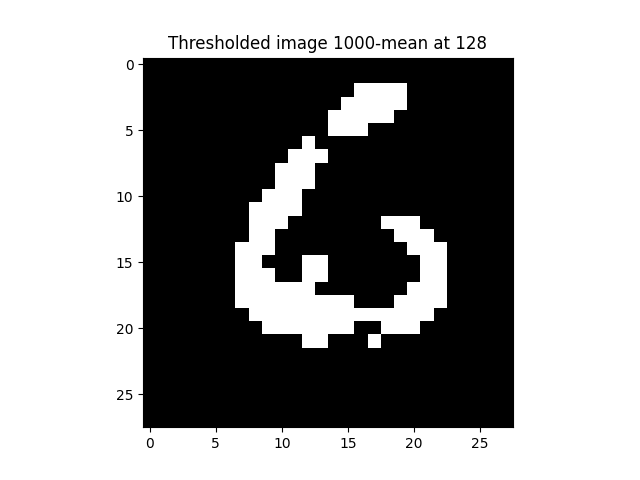
\includegraphics[width=0.35\textwidth]{image9.png}
\captionof{figure}{Square of the subtraction of experiment image and mean image for experiment 1000\label{fig:image9}}
\end{center}

\begin{center}
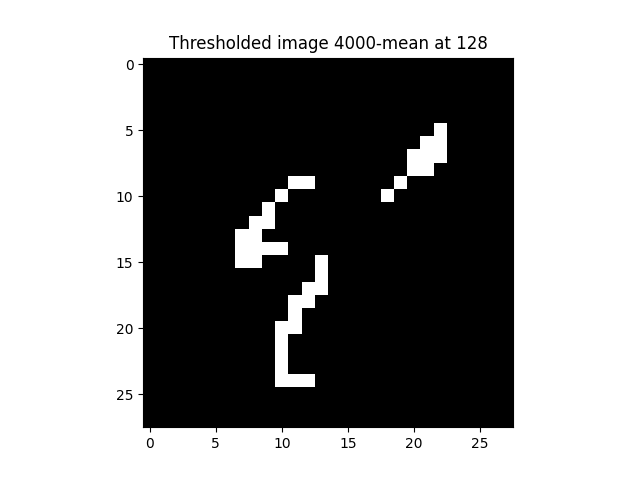
\includegraphics[width=0.35\textwidth]{image10.png}
\captionof{figure}{Square of the subtraction of experiment image and mean image for experiment 4000\label{fig:image10}}
\end{center}

Now that the subtraction of the experiment image and the mean image has occurred, the resultant value is squared. Refer to figure 9 and Figure 10 for the graphical results.

\begin{center}
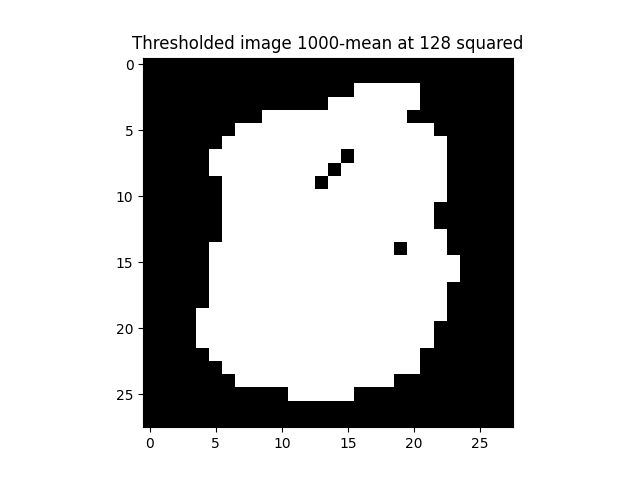
\includegraphics[width=0.35\textwidth]{image11.png}
\captionof{figure}{Square of the subtraction of experiment image and mean image for experiment 1000\label{fig:image9}}
\end{center}

\begin{center}
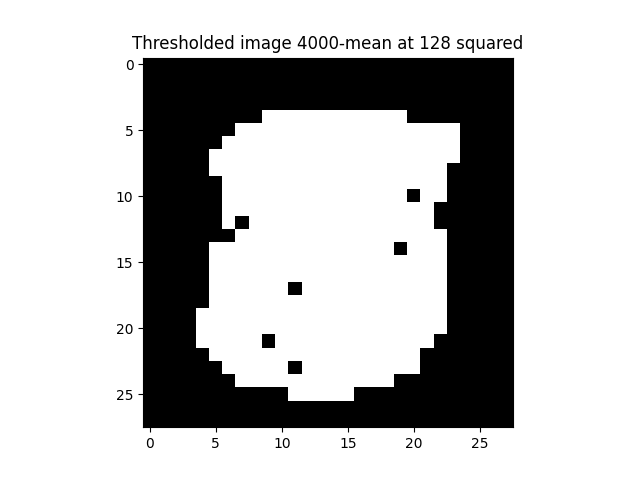
\includegraphics[width=0.35\textwidth]{image12.png}
\captionof{figure}{Square of the subtraction of experiment image and mean image for experiment 4000\label{fig:image10}}
\end{center}

The final step is to sum the values of the squared subtraction of the experiment image and the mean image. The results are shown in figure 11 and figure 12.

The images of the power spectral density plots by class will listed in the following ten figures.


\begin{center}
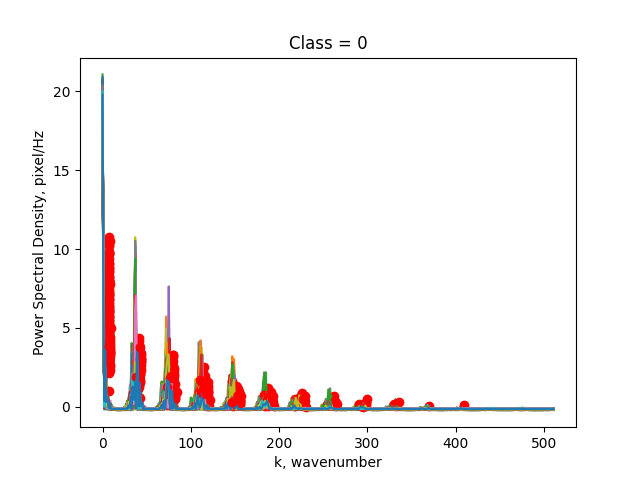
\includegraphics[width=0.35\textwidth]{fft_0.png}
\captionof{figure}{PSD of Class 0 handwriting data}
\end{center}

\begin{center}
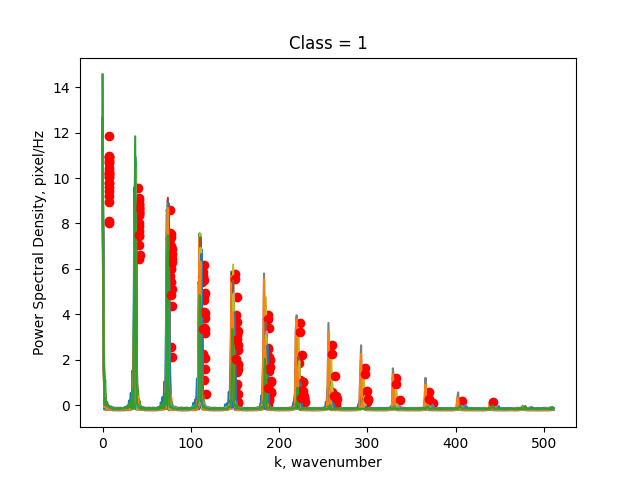
\includegraphics[width=0.35\textwidth]{fft_1.png}
\captionof{figure}{PSD of Class 1 handwriting data}
\end{center}

\begin{center}
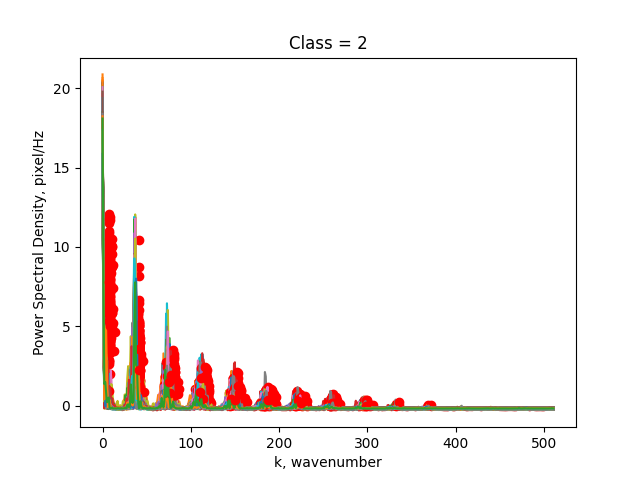
\includegraphics[width=0.35\textwidth]{fft_2.png}
\captionof{figure}{PSD of Class 2 handwriting data}
\end{center}

\begin{center}
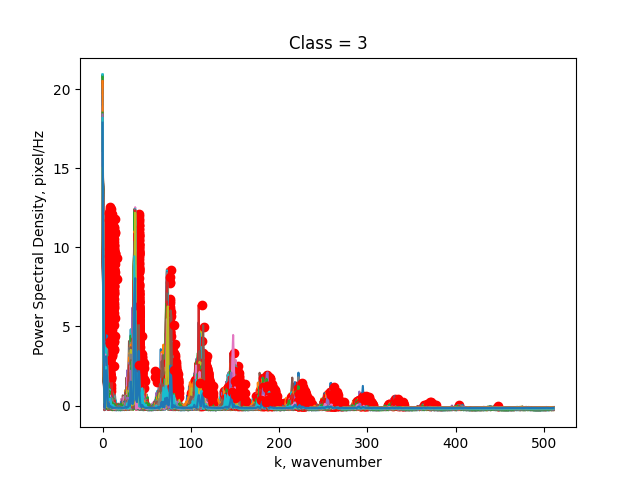
\includegraphics[width=0.35\textwidth]{fft_3.png}
\captionof{figure}{PSD of Class 3 handwriting data}
\end{center}

\begin{center}
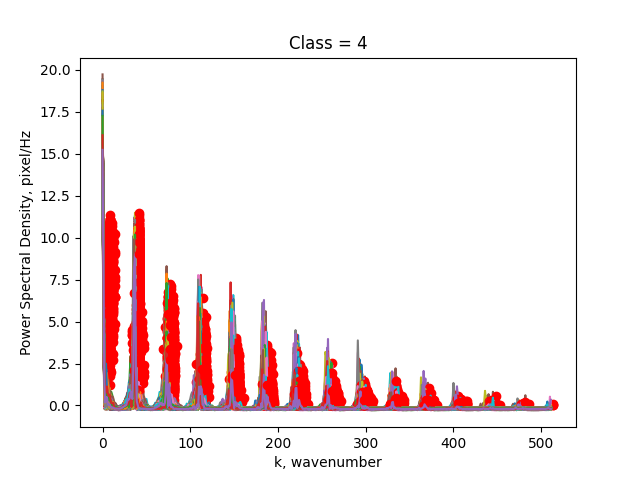
\includegraphics[width=0.35\textwidth]{fft_4.png}
\captionof{figure}{PSD of Class 4 handwriting data}
\end{center}

\begin{center}
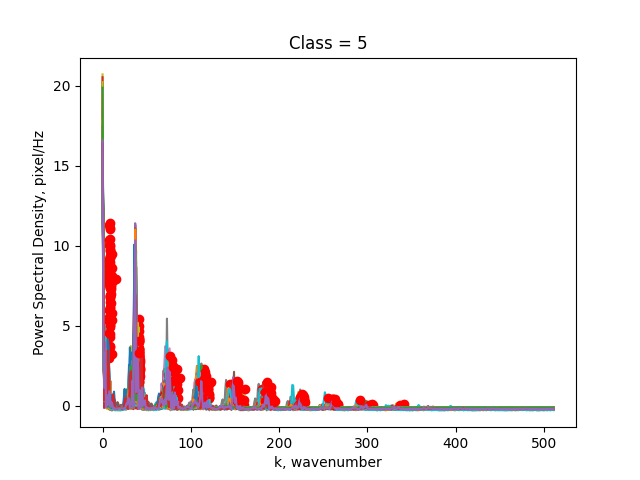
\includegraphics[width=0.35\textwidth]{fft_5.png}
\captionof{figure}{PSD of Class 5 handwriting data}
\end{center}

\begin{center}
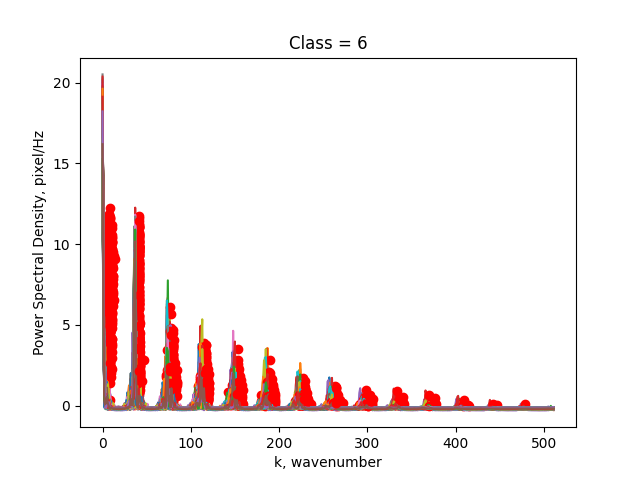
\includegraphics[width=0.35\textwidth]{fft_6.png}
\captionof{figure}{PSD of Class 6 handwriting data}
\end{center}

\begin{center}
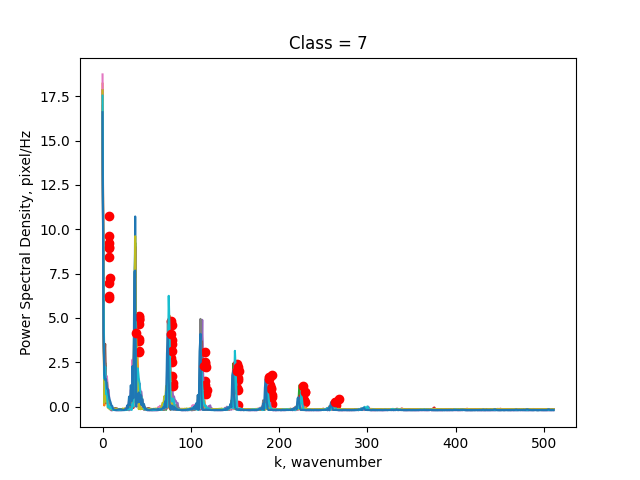
\includegraphics[width=0.35\textwidth]{fft_7.png}
\captionof{figure}{PSD of Class 7 handwriting data}
\end{center}

\begin{center}
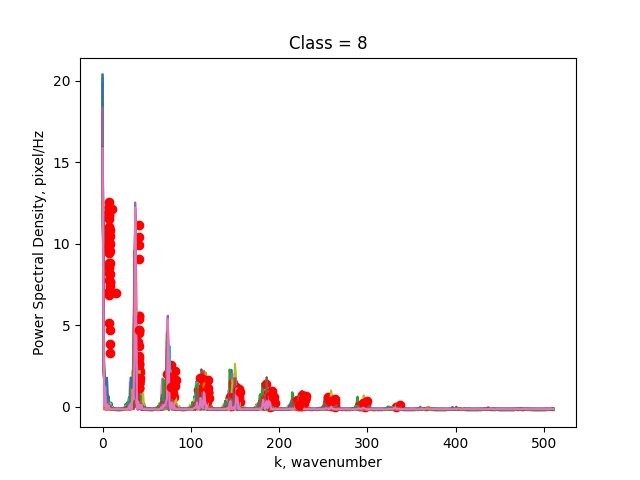
\includegraphics[width=0.35\textwidth]{fft_8.png}
\captionof{figure}{PSD of Class 8 handwriting data}
\end{center}
    

\begin{center}
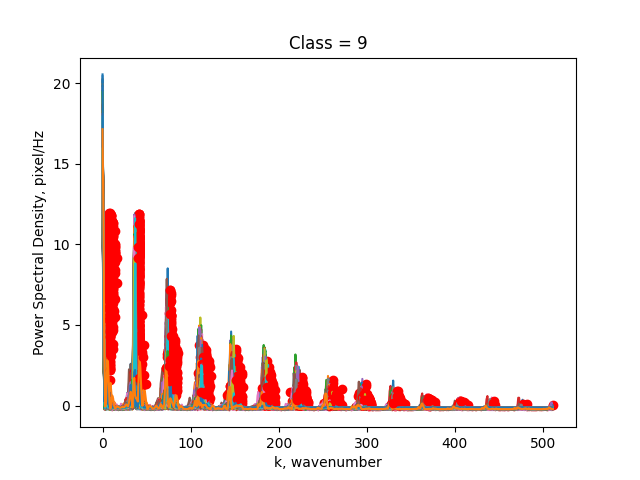
\includegraphics[width=0.35\textwidth]{fft_9.png}
\captionof{figure}{PSD of Class 9 handwriting data}
\end{center}


\begin{center}
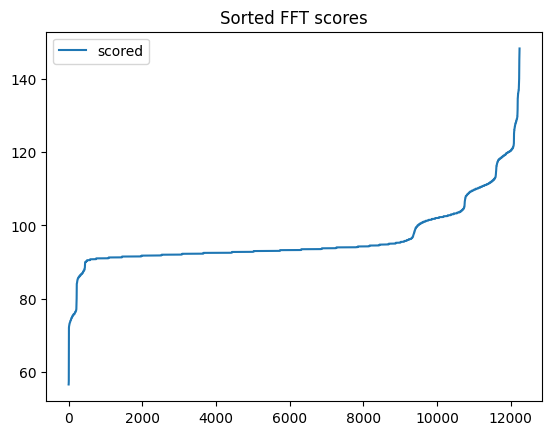
\includegraphics[width=0.35\textwidth]{sorted_fft_scores.png}
\captionof{figure}{Sorted FFT scores}
\end{center}

    
        